\chapter{Praktická část}

\section{Popis dat}\label{sec:popisdat}

Poskytovatelem dat je Datové centrum Ústeckého kraje (DCÚK), které spravuje a~zpřístupňuje data z~různých systémů veřejné správy.
Jedná se o~záznamy ze systému pro sledování pohybu vozidel správy a~údržby silnic. 

Samotný dataset má velikost přibližně 650 MB a~obsahuje zhruba 600 tisíc záznamů. Data jsou uložena v~tabulkové struktuře ve formátu CSV.
Obsahuje celkem 54 atributů různých datových typů. Převládají celočíselné a~desetinné hodnoty, které reprezentují měřené nebo stavové veličiny, dále textové atributy sloužící především jako identifikátory a~časové údaje. 
Struktura dat je převážně plochá, přičemž každý řádek představuje jeden záznam o~stavu vozidla v~konkrétním časovém okamžiku.

Tyto informace umožňují analýzu pohybu vozidel v~čase a~prostoru, například pro vyhodnocení efektivity údržby silniční sítě nebo sledování tras jednotlivých vozidel.

\section{Předběžná srovnávací analýza systémů}\label{sec:db_overview}
Pro účely experimentálního porovnání bylo vybráno osm databázových systémů reprezentujících různé přístupy k~ukládání a~zpracování dat. 
Výběr zahrnuje relační, sloupcové, dokumentové i~specializované databáze pro časové řady, tak i~databáze, které nejsou přímo určené pro ukládání časových řad.
Zastoupeny jsou systémy optimalizované pro transakční zpracování (OLTP), analytické zpracování (OLAP) i~databáze kombinující vlastnosti obou přístupů.

Následující tabulka uvádí základní klasifikaci vybraných systémů podle kategorie, typu pracování, způsobu ukládání dat, podporovaného dotazovacího jazyka a použité licence.
Podrobnější popis architektury, principů ukládání a specifických vlastností každého z uvedených systémů je pak předmětem samostatných podkapitol.

\begin{table}[H]
\centering
\footnotesize
\setlength{\tabcolsep}{3pt}
\renewcommand{\arraystretch}{1.25}

\begin{tabular}{|l|l|l|l|l|l|}
\hline
\textbf{DB} & \textbf{Kategorie} & \textbf{Typ} & \textbf{Storage} & \textbf{Jazyk} & \textbf{Licence} \\
\hline
Apache IoTDB & TSDB & Hybrid& TsFile & IoTDB-SQL & Apache 2.0 \\
\hline
ClickHouse & Sloupcová & OLAP & MergeTree & SQL & Apache 2.0 \\
\hline
InfluxDB 3 & TSDB & Hybrid & Parquet + Object store & SQL & OSS / Enterprise \\
\hline
MariaDB & RDBMS & OLTP & Různé & SQL & GPLv2 \\
\hline
MariaDB ColumnStore & Sloupcová & OLAP & ColumnStore Engine & SQL & GPLv2 \\
\hline
MongoDB & Dokumentová & OLTP & WiredTiger & MQL & SSPL \\
\hline
QuestDB & TSDB & Hybrid & Sloupcový formát & SQL & Apache 2.0 \\
\hline
TimescaleDB & TSDB & Hybrid & Hypertables & SQL & Apache 2.0 \\
\hline
\end{tabular}

\caption{Srovnání databázových systémů}
\label{table:db_compact}
\end{table}

\subsection{Apache IoTDB}

Apache IoTDB\footnote{https://iotdb.apache.org} je časově orientovaná databáze navržená specificky pro správu velkých objemů časových řad generovaných v~prostředí Internetu věcí (IoT) a~průmyslového internetu věcí (IIoT). 
Projekt vznikl na univerzitě Tsinghua v~Pekingu pod vedením profesora Jianmina Wanga, kde tým od roku 2011 řešil problémy s~ukládáním masivních strojových dat a~v~roce 2016 formálně představil vlastní formát TsFile a~na jeho základě vyvinul databázi IoTDB. 
\cite{iotdbdocs}

Hlavním důvodem vzniku IoTDB byla neschopnost existujících NoSQL i~relačních databází efektivně zpracovávat specifika průmyslových časových řad: extrémně vysokou frekvenci zápisu z~milionů senzorů, potřebu vysoké komprese při~zachování přesnosti, zpožděná data a~požadavek na analytiku přímo na okrajových zařízeních. 
\cite{iotdbdocs}

Z~pohledu ukládání dat využívá IoTDB vlastní sloupcový formát TsFile, optimalizovaný pro časové řady. 
Data jsou nejprve zapisována do paměťové struktury (\textit{memtable}) a~zajištěna transakčním logem (WAL). 
Následně jsou převedena do neměnných souborů TsFile na disku. 
Celková organizace vychází z~LSM-based přístupu, který je koncepčně podobný struktuře popsané v~kapitole \ref{lsm_tree}. 
Díky specifickým kompresním a~kódovacím technikám pro časové řady dosahuje IoTDB vysokých kompresních poměrů při~zachování rychlého zápisu i~čtení. 
\cite{iotdbdocs}

Systém je architektonicky rozdělen do dvou hlavních komponent:

\begin{itemize}
    \item \textbf{ConfigNode} \\
    Spravuje metadata clusteru\footnote{\textit{Cluster} - skupina uzlů, které spolupracují a~fungují jako jeden logický celek}, schéma časových řad a~koordinaci distribuovaných uzlů. 
    Zajišťuje jednotný stav mezi uzly a~vysokou dostupnost v~režimu clusteru.
    
    \item \textbf{DataNode} \\
    Zajišťuje vlastní zpracování dotazů a~úložiště dat. 
    Každý DataNode uchovává fyzická data ve formátu TsFile a~provádí lokální výpočetní operace nad přidělenými časovými řadami.
\end{itemize}

Architektura umožňuje horizontální škálování přidáváním DataNode, čímž se zvyšuje jak kapacita úložiště, tak propustnost zpracování dotazů.

Databáze podporuje SQL-like dotazovací jazyk (IoTDB-SQL), který rozšiřuje standardní SQL o~funkce specifické pro časové řady, jako je \texttt{LAST} dotaz pro okamžité získání nejnovější hodnoty senzoru s~mikrosekundovou latencí. 

IoTDB je dostupné jako open-source projekt pod licencí Apache 2.0 pro self-hosting, a~to jak v~samostatném, tak v~distribuovaném režimu. 

\subsection{ClickHouse}

ClickHouse\footnote{https://clickhouse.com} je sloupcově orientovaná databáze určená pro analytické dotazy v~reálném čase (OLAP), původně vyvinutá společností Yandex jako interní nástroj pro zpracování velkých objemů dat. 
Později byla uvolněna jako open-source projekt a~postupně se stala jednou z~populárních databází pro analytické zpracování dat. \cite{clickhouseintro}

Hlavním důvodem vzniku ClickHouse byla potřeba efektivního zpracování a~analýzy rozsáhlých logových a~telemetrických dat v~reálném čase, kde tradiční relační databáze nedokázaly splnit požadavky na výkon.

Významnou vlastností ClickHouse je využití vektorového zpracování dotazů a~sloupcového uložení dat, které umožňuje efektivně provádět agregace nad rozsáhlými datovými sadami. 
Díky tomu je vhodný zejména pro analytické scénáře, jako jsou datové sklady, analýza logů nebo zpracování telemetrických dat.

ClickHouse je dostupný jak ve formě open-source řešení pro self-hosting, tak i~jako plně spravovaná cloudová služba. Open-source varianta umožňuje nasazení na vlastních serverech nebo v~libovolném cloudovém prostředí.

Z~pohledu ukládání dat využívá ClickHouse vlastní rodinu úložných systémů založených na technologii \textit{MergeTree}. 
Ta je koncepčně podobná struktuře LSM Tree popsané v~kapitole \ref{lsm_tree}. \cite{clickhousearchitecture}

Databáze podporuje standardní jazyk SQL rozšířený o~analytické a~časové funkce. Dále podporuje jazyky jako jsou PRQL (Pipelined Relational Query Language), nebo KQL (Kusto Query Language). \cite{clickhousearchitecture}

Databáze je licencovaná pod Apache License 2.0\footnote{https://www.apache.org/licenses/LICENSE-2.0}, což umožňuje široké využití a~přizpůsobení v~různých projektech a~prostředích.

\subsection{InfluxDB 3}

InfluxDB 3\footnote{https://www.influxdata.com} je časově orientovaná databáze (TSDB) navržená pro ukládání a~analýzu dat závislých na čase, například metrik, senzorických dat nebo logů.

Vznikla v~roce 2013 společností InfluxData.
Je optimalizována pro vysokou rychlost zápisu a~práci s~časovými intervaly, což ji činí vhodnou pro IoT, monitoring a~observabilitu systémů. 
\cite{influxdbdocs}

InfluxDB nyní využívá hlavně jazyk SQL, v~minulosti ovšem ale využíval vlastní dotazovací jazyky InfluxQL a~následně Flux. V~nejnovějších verzích podpora pro Flux už není.
Kromě toho je dostupný také HTTP API\footnote{\textit{API} - Application Programming Interface, rozhraní, přes které spolu komunikují různé aplikace.} přístup. 
\cite{influxdbdocs}

Nejnovější verze InfluxDB 3 je postavena na tzv. FDAP stacku\footnote{\textit{FDAP} - Flight, DataFusion, Arrow, Parquet, sada open-source komponent Apache Software Foundation, které tvoří jádro systému.}, což umožňuje zaměřit vývoj na časově specifické funkce místo reinplementace nízkoúrovňových databázových komponent. \cite{influxdbdocs}

Základní stavební kameny architektury jsou:

\begin{itemize}
    \item \textbf{Apache Arrow} \\
    Efektivní sloupcový formát pro reprezentaci dat v~operační paměti. Umožňuje rychlé zpracování dat a~efektivní sdílení mezi různými aplikacemi bez nutnosti kopírování. \cite{influxdbdocs}
    \item \textbf{Apache Parquet} \\
    Sloupcový formát pro trvalé uložení dat v~objektovém úložišti. Optimalizovaný pro analytické dotazy a~umožňují efektivní kompresi a~ukládání velkých objemů dat. \cite{apacheparquet}
    \item \textbf{Apache DataFusion} \\
    Modulární analytický query engine napsaný v~Rust, který využívá Arrow jako paměťový model. Poskytuje podporu pro SQL, InfluxQL i~vlastní analytické operace, včetně JOINů a~subdotazů. \cite{influxdbdocs}
    \item \textbf{Apache Arrow Flight} \\
    Síťový protokol pro rychlý přenos dat ve formátu Apache Arrow mezi servery a~klienty. Podporuje také standard Arrow Flight SQL, díky kterému lze k~databázi přistupovat prostřednictvím rozhraní JDBC\footnote{\textit{JDBC (Java Database Connectivity)} - standardní API pro připojení aplikací v~jazyce Java k~databázím} a~ODBC\footnote{\textit{ODBC (Open Database Connectivity)} - standardní API pro připojení aplikací k~databázím nezávisle na použitém programovacím jazyce a~databázovém systému}. 
    \cite{influxdbdocs}
\end{itemize}

InfluxDB 3 je optimalizována především pro write-heavy zátěž, tedy scénáře s~velmi vysokou frekvencí zápisu časově označených dat. 
Naopak komplexní analytické dotazy nad velmi rozsáhlými historickými daty mohou být méně efektivní.

Z~pohledu ekosystému je InfluxDB 3 často využívána společně s~nástroji Telegraf a~Grafana, pro které existuje oficiální datový zdrojový plugin umožňující přímé napojení a~vizualizaci dat.

InfluxDB 3 je dostupná ve více edicích, od open-source InfluxDB 3 Core až po placené varianty jako InfluxDB 3 Enterprise a~cloudové služby. 
Pokročilé funkce, například vysoká dostupnost, clustering\footnote{\textit{Clustering} - technika, která seskupuje záznamy podle jejich podobnosti nebo klíče, aby se fyzicky ukládaly blízko sebe a~tím se zrychlilo jejich následné vyhledávání} nebo produkční škálování, jsou typicky součástí Enterprise nebo cloudových verzí, zatímco Core je určený pro single-node a~neprodukční použití. 
Licenční a~funkční rozsah se liší podle zvolené edice, nicméně open-source varianta InfluxDB 3 Core je dostupná pod licencí MIT\footnote{https://opensource.org/licenses/MIT} nebo Apache License 2.0\footnote{https://www.apache.org/licenses/LICENSE-2.0}.

\subsection{MariaDB}

MariaDB\footnote{https://mariadb.org} je open-source relační databázový systém vyvinutý jako komunitní nástupce MySQL. Vznikla v~roce 2009 jako reakce na akvizici Sun Microsystems (a~s~ním i~MySQL) společností Oracle. 
Cílem projektu bylo zachovat svobodnou a~otevřenou licenční politiku, zároveň však poskytnout plnou kompatibilitu s~existujícími MySQL aplikacemi a~postupně rozšiřovat funkcionalitu nad rámec původního systému.
\cite{mariadbdocs}

Z~architektonického hlediska využívá MariaDB modulární koncept pluggable storage engine, což umožňuje volit optimální způsob ukládání dat podle charakteru úlohy. 
Vedle standardního InnoDB (který zajišťuje transakční zpracování a~vnější klíče) jsou dostupné například Aria pro rychlé tabulky bez nutnosti transakcí, MyRocks založený na technologii RocksDB pro efektivní zápis, nebo Spider pro horizontální dělení dat napříč více servery.

Databázový server zpracovává dotazy v~jazyce SQL a~podporuje pokročilé konstrukce jako jsou common table expressions (CTE), okénkové funkce, dotazy přes JSON datové typy a~geoprostorové indexy.
\cite{mariadbdocs}

MariaDB je šířena pod licencí GNU General Public License verze 2\footnote{https://www.gnu.org/licenses/old-licenses/gpl-2.0.cs.html}, což zaručuje svobodné použití, studium i~modifikaci zdrojových kódů. 
Systém je dostupný ve formě komunitní edice MariaDB Community Server, která je vhodná pro většinu produkčních i~vývojových scénářů. 
Pro organizace s~požadavkem na profesionální podporu, pokročilé zabezpečení nebo správu existuje placená MariaDB Enterprise.

\subsection{MariaDB ColumnStore}
MariaDB ColumnStore\footnote{https://mariadb.com/docs/analytics/mariadb-columnstore} je sloupcové rozšíření pro relační databázi MariaDB, navržené pro analytické zpracování velkých objemů dat (OLAP) a~hybridní transakčně-analytické zpracování (HTAP). 
Původně vychází z~projektu InfiniDB společnosti Calpont, který byl v~roce 2014 uvolněn pod open-source licencí a~následně integrován do ekosystému MariaDB.
\cite{mariadbcolumnstore}

Na rozdíl od samostatných analytických databází je ColumnStore plně integrován do MariaDB Serveru jako plugin storage engine. 
To umožňuje v~rámci jedné instance kombinovat transakční tabulky v~InnoDB a~analytické tabulky v~ColumnStore, případně provádět cross-engine JOINy mezi oběma typy úložišť.
\cite{mariadbcolumnstore}

Z~pohledu dotazování podporuje ColumnStore standardní SQL včetně agregací, okenních funkcí a~komplexních JOINů. 
Pro rychlý bulk load dat je k~dispozici nástroj cpimport, který obchází SQL vrstvu a~zapisuje data přímo do sloupcového úložiště, což minimalizuje režii při~importu velkých datasetů. 
\cite{mariadbcolumnstore}

Systém je rozdělen do dvou hlavních typů komponent:

\begin{itemize}
\item \textbf{User Modules (UM)} \
Slouží jako vstupní bod systému a~zajišťují SQL engine, správu připojení a~orchestraci dotazů. 
User Module přijme SQL dotaz, provede jeho analýzu a~rozdělí jej na dílčí operace, které jsou následně distribuovány do výpočetních uzlů. 
Zároveň může provádět operace, které nelze paralelizovat, a~vrací finální výsledky zpět klientovi prostřednictvím MariaDB serveru.

\item \textbf{Performance Modules (PM)} \\
Zajišťují samotné distribuované zpracování dat. 
Každý Performance Module provádí výpočetní operace nad přidělenou částí dat, která je uložena ve sloupcové formě. 
PM uzly čtou a~zapisují data z~columnar storage a~vracejí mezivýsledky zpět User Module.

\end{itemize}

Architektura je plně škálovatelná horizontálně, přidáním PM se zvyšuje výkon zpracování dotazů, zatímco přidáním UM se zvyšuje propustnost a~dostupnost systému. 
Každý uzel je navíc vícevláknový, což dále zvyšuje výkon na úrovni jednotlivých serverů.

Z~pohledu ukládání dat využívá MariaDB ColumnStore sloupcový model, kde jsou data ukládána po sloupcích namísto řádků. 
Tento přístup umožňuje číst pouze relevantní sloupce pro daný dotaz, čímž se výrazně snižuje objem načítaných dat. 
Řádky jsou logicky rekonstruovány pomocí offsetů napříč sloupcovými soubory. 
Horizontální škálování je dosaženo rozdělením dat mezi PM, zatímco další optimalizace čtení je zajištěna pomocí Extent Map, které obsahují metadatové informace o~rozsazích dat a~umožňuje přeskočení nerelevantních bloků.

Jakožto modul pro MariaDB také spadá pod licenci GNU General Public License verze 2.
\subsection{MongoDB}

MongoDB\footnote{https://www.mongodb.com} je dokumentově orientovaná NoSQL databáze navržená pro ukládání a~zpracování velkých objemů nestrukturovaných a~polostrukturovaných dat. 
Vznikla v~roce 2009 společností 10gen (dnes MongoDB Inc.) jako odpověď na rostoucí potřebu flexibilního datového modelu, který by lépe reflektoval strukturu moderních aplikací a~umožnil horizontální škálování bez komplexních změn schématu. 
\cite{mongodbdocs}

Hlavním důvodem vzniku MongoDB byla neschopnost relačních databází efektivně zpracovávat rychle se měnící data s~proměnlivou strukturou, zejména v~kontextu webových aplikací a~real-time systémů, kde je požadována vysoká propustnost zápisu a~jednoduchá distribuce dat napříč servery.
\cite{mongodbdocs}

Z~pohledu ukládání dat využívá MongoDB formát BSON. 
Data jsou organizována do kolekcí, které obsahují jednotlivé dokumenty s~flexibilním schématem. 
Každý dokument může mít odlišnou strukturu. 
Pro trvalé uložení na disk využívá výchozí storage engine WiredTiger\footnote{WiredTiger podporuje jak řádko    vé, tak sloupcové ukládání dat. Tato schémata je schopný aplikovat i~přímo na úrovni kolekcí. 
Využívá jak LSM stromy (viz \ref{lsm_tree}), tak i~B-Tree struktury (viz \ref{btree}).
\cite{wiredtiger}}, která podporuje kompresi, šifrování a~řízení souběžnosti na úrovni dokumentů. \cite{mongodbdocs}

Z~pohledu dotazování používá MongoDB vlastní dotazovací jazyk MQL (MongoDB Query Language), který umožňuje vyhledávání dokumentů na základě jejich struktury, obsahu i~vnořených polí. 
Kromě základních CRUD\footnote{\textit{CRUD} - Create, Read, Update, Delete, základní operace databázových systémů} operací podporuje komplexní transformace a~výpočty přímo v~databázi, textové vyhledávání, geoprostorové dotazy a~operace nad časovými řadami. 
\cite{mongodbdocs}

MongoDB je dostupný ve více edicích. 
Komunitní edice MongoDB Community Server je šířena pod licencí SSPL (Server Side Public License)\footnote{https://www.mongodb.com/legal/licensing/server-side-public-license}, která umožňuje volné použití a~modifikace při~splnění určitých podmínek pro cloudové nasazení. 
Pro komerční použití s~pokročilými funkcemi, jako je in-memory engine, šifrování na úrovni databáze nebo auditování, je určena placená MongoDB Enterprise Edition. 
Kromě toho je nabízena plně spravovaná cloudová služba MongoDB Atlas, která poskytuje automatizované zálohování, monitoring a~globální distribuci dat. 
\cite{mongodbdocs}

\subsection{QuestDB}
QuestDB\footnote{https://questdb.com} je sloupcově orientovaná databáze určená pro časové řady a~analytické úlohy v~reálném čase, původně vyvinutá jako interní nástroj pro sledování plavidel v~energetickém obchodním domě v~roce 2012. 
Později byl projekt přepracován na open-source databázi a~oficiálně uveden v~roce 2019. 
Hlavním důvodem vzniku byla potřeba zpracovávat vysokofrekvenční data s~mikrosekundovou latencí, kde tradiční databáze nedokázaly zajistit požadovanou propustnost zápisu a~rychlost dotazů.
\cite{questdbdocs}

Z~pohledu ukládání dat využívá QuestDB sloupcový model založený na relačních tabulkách s~typovanými sloupci a~označeným časovým razítkem. 
Příchozí data jsou nejprve zapisována do transakčního logu (WAL). 
Následně jsou převedena do nativního sloupcového binárního formátu s~rozložením souborů podle sloupců a~časových partitionů, což umožňuje dotazům číst pouze relevantní sloupce a~časové úseky. 
Dotazy jsou dále optimalizovány pro rychlé vektorizované agregace. 
Starší data mohou být automaticky přesunuta do úložiště objektů ve formátu Apache Parquet.
\cite{questdbdocs}

QuestDB podporuje standardní SQL rozšířený o~časové funkce. 
Pro vysokorychlostní ingestování je k~dispozici protokol InfluxDB Line Protocol, zatímco pro dotazování implementuje PostgreSQL wire protocol, což umožňuje připojení standardními PostgreSQL klienty bez nutnosti speciálních ovladačů. 
K~dispozici je také REST API a~vestavěná webová konzole.

QuestDB je dostupný jako open-source projekt pod licencí Apache License 2.0 a dále i jako QuestDB Enterprise. Ta disponuje funkcemi, které přidávjí možnost replikace dat, automatického zálohování, horizontální škálování, a podporu úložiště nad objektovým storage (např. S3, Azure Blob Storage nebo GCS).

\subsection{TimescaleDB}

TimescaleDB\footnote{https://www.tigerdata.com} je open-source relační databázový systém rozšířený o~schopnosti pro práci s~časovými řadami a~analytické zpracování, implementovaný jako rozšíření pro PostgreSQL. 
Projekt vznikl v~roce 2015 z~akademického výzkumu na univerzitě Princeton, přičemž první veřejná verze byla uvedena v~roce 2017. 
Hlavním motivem bylo vytvořit systém, který by spojil výhody tradičních relačních databází, plnou podporu SQL, transakční konzistenci a~bohatý ekosystém nástrojů, s~výkonem specializovaných databází pro časové řady, aniž by bylo nutné opouštět osvědčenou platformu PostgreSQL. 
\cite{timescaledbdocs}

Pro ukládání dat využívá TimescaleDB koncept hypertables, abstrakce nad standardní PostgreSQL tabulkou, která je automaticky rozdělena do menších časových segmentů (chunků), přičemž pro uživatele i~aplikace zůstává viditelná jako jediná logická tabulka.
Data jsou rozdělována do chunků na základě časového sloupce a~volitelně i~prostorového klíče.
Proti výpadkům implementuje transakční log (WAL).

Systém podporuje plný standardní SQL prostřednictvím PostgreSQL, rozšířený o~časové funkce pro pokročilou analytiku. 
Klíčovou vlastností jsou continuous aggregates, které automaticky předpočítávají agregace na pozadí a~umožňují tak real-time analytiku nad obrovskými datovými sadami. 
Díky implementaci jako PostgreSQL extension je plně kompatibilní s~existujícími PostgreSQL nástroji, ovladači~a~ekosystémem. 
\cite{timescaledbdocs}

TimescaleDB je šířen pod licencí Apache License 2.0, což umožňuje volné použití i~modifikace. 
Systém je dostupný jako open-source rozšíření pro self-hosting na vlastních serverech. 
Pro produkční prostředí s~požadavkem na automatizované zálohování, monitoring a~horizontální škálování je nabízena plně spravovaná cloudová služba Timescale Cloud, dostupná na platformách AWS, Azure a~GCP. 
Dále existuje i TimescaleDB Enterprise, která oproti open-source edici poskytuje rozšířené podnikové funkce, zejména pokročilou podporu, SLA\footnote{\textit{SLA (Service Level Agreement)} – dohoda o úrovni poskytovaných služeb, která definuje garantované parametry podpory, například dostupnost služby, dobu odezvy a řešení incidentů}, nástroje pro vysokou dostupnost, bezpečnost a monitorování.
\cite{timescaledbdocs}

\section{Návrh testovacího scénáře}
V~následujících odstavcích popíši~realizace a~návrhy testovacího prostředí, které jsem využil pro porovnání jednotlivých databázových systémů.
V~mém prostředí chci zadefinovat co nejbližší jednotné prostředí, jako jsou například stejná data a~stejné HW prostředky.
To budu realizovat pomocí orchestrace založené na Ansible. 
Monitoring běhu jednotlivých kontejnerů je založen na systému Prometheus a~sesbíraná HW data budou vizualizována pomocí nástroje Grafana.

\subsection{Testovací prostředí}
Pro realizaci experimentů byl zvolen operační systém Ubuntu Server v~konfiguraci CLI (Command Line Interface) bez grafického prostředí. 
Důvodem této volby byla především snaha minimalizovat režii operačního systému a~zajistit co největší podíl hardwarových prostředků pro samotné databázové systémy. 
Současně jde o~stabilní a~široce podporovanou linuxovou distribuci běžně používanou v~serverových prostředích.

Ubuntu Server standardně poskytuje virtualizační platformu LXD, která umožňuje vytváření jak systémových kontejnerů, tak virtuálních strojů. 
Pro účely této práce byly využity kontejnery, protože poskytnutá architektura od DCÚK nepodporuje vytváření virtuálních strojů. 
Díky tomu lze jednotlivé databázové systémy provozovat v~navzájem nezávislých prostředích bez rizika vzájemného ovlivňování. 

Současně LXD umožňuje rychlé vytváření, konfiguraci i~odstraňování kontejnerů, což výrazně usnadňuje opakovatelnost experimentů a~zajišťuje, že všechny databázové systémy byly testovány za srovnatelných podmínek.

\subsection{Automatizace nasazení}
Pro automatizaci přípravy testovacího prostředí byl zvolen nástroj Ansible. 
Hlavním důvodem byla jeho agent-less architektura, která nevyžaduje instalaci žádného trvale běžícího agenta na spravovaných systémech.

Vzhledem k~tomu, že jednotlivé kontejnery vznikaly pouze po dobu experimentů a~po jejich dokončení byly odstraněny, by instalace a~správa agentů představovala zbytečnou režii. 
Ansible komunikuje prostřednictvím protokolu SSH a~konfiguraci provádí pouze při~spuštění jednotlivých úloh. 
Tento přístup umožňuje jednoduše opakovat celé nasazení, zajišťuje reprodukovatelnost experimentů a~současně minimalizuje vliv automatizační vrstvy na měřené výsledky.

Další výhodou je možnost popsat kompletní infrastrukturu pomocí Infrastructure as Code, díky čemuž lze všechny experimenty kdykoliv znovu vytvořit ve stejné konfiguraci.

\subsection{Monitorování}
Pro sledování průběhu experimentů byl zvolen monitorovací stack tvořený nástroji Prometheus a~Grafana.

Prometheus zajišťuje pravidelný sběr systémových metrik prostřednictvím pull modelu, který dobře odpovídá charakteru testovacího prostředí a~vzhledem k~tomu, že hlavní komponenta běží na jiném stroji než databázové systémy, přidává menší režii. 
Během experimentů byly sledovány zejména metriky využití procesoru, operační paměti, diskových operací a~dalších systémových prostředků.

Grafana sloužila jako vizualizační vrstva, která umožnila průběžně sledovat chování jednotlivých databázových systémů během testů a~současně usnadnila následnou analýzu naměřených dat. 

\section{Konfigurace testovacího prostředí a~databázových systémů}

Tato kapitola popisuje konfiguraci testovacího prostředí a~jednotlivých databázových systémů použitých při~experimentech. 
Cílem bylo zajistit srovnatelné podmínky pro všechny testované databáze a~minimalizovat vliv rozdílného nastavení na výsledky měření. 
Následující podkapitoly se věnují instalaci Ansible, architektuře prostředí a~ukázkové konfiguraci databázového systému ClickHouse.

\subsubsection{Instalace}
Ansible byl nainstalován pouze na řídicím stroji, tedy na notebooku, ze kterého je spouštěna veškerá orchestrace. 
Díky agent-less architektuře není potřeba instalovat žádnou komponentu přímo na testovaných kontejnerech, ty vyžadují pouze funkční SSH server a~Python 3, což je zajištěno již při~jejich vytváření.

Instalace na řídicím stroji s~Ubuntu byla provedena pomocí balíčkovacího systému \texttt{apt}:

\begin{lstlisting}[caption={Instalace Ansible}, label={lst:ansibleinstall}, captionpos=b]
sudo apt update
sudo apt install -y ansible
\end{lstlisting}

Vzhledem k~tomu, že vytváření a~správa kontejnerů je realizována přes LXD, bylo nutné doinstalovat kolekci \texttt{community.general} (často již ale bývá přímo v~balíčku Ansible), která poskytuje modul \texttt{lxd\_container} používaný v~roli \texttt{common-create} (viz podsekce \ref{sec:rolecommon}):

\begin{lstlisting}[caption={Instalace kolekce community.general}, label={lst:communitygeneral}, captionpos=b]
ansible-galaxy collection install community.general
\end{lstlisting}

\subsection{Architektura}
Každý testovaný databázový systém běží ve svém samostatném LXD kontejneru, který je nakonfigurován s~přidělenými hardwarovými prostředky (CPU, RAM, diskový prostor).

Při~vytvoření kontejneru se do něj nainstaluje zvolený databázový systém a~Node Exporter pro sběr metrik.

Na vyhrazeném kontejneru běží Grafana a~Prometheus, které zajišťují sběr a~vizualizaci metrik z~jednotlivých kontejnerů.
\clearpage
\subsubsection{Ansible Inventář}
Inventář definuje cílové hosty a~je rozdělen do tří skupin. 
Pro pilotní i~lokální testování je použit soubor \texttt{inventory/local}, který odpovídá síti vytvářené LXD na notebooku:

\begin{lstlisting}[language=YAML, caption={inventory/local}, label={lst:inventorylocal}, captionpos=b]
databases:
  vars:
    ansible_connection: ssh
  hosts:
    mariadb:
      ansible_host: 10.187.240.2
    questdb:
      ansible_host: 10.187.240.3
    influxdb:
      ansible_host: 10.187.240.4
    iotdb:
      ansible_host: 10.187.240.5
    clickhousedb:
      ansible_host: 10.187.240.6
    timescaledb:
      ansible_host: 10.187.240.7
    columnstoredb:
      ansible_host: 10.187.240.8
    mongodb:
      ansible_host: 10.187.240.9

monitoring:
  hosts:
    grafana:
      ansible_host: 10.187.240.240

servers:
  hosts:
    localhost:
      ansible_host: localhost
      ansible_connection: local
\end{lstlisting}
\clearpage
Skupina \textbf{databases} obsahuje osm hostů, jeden pro každý testovaný databázový systém, se staticky přidělenou IP adresou uvnitř lokální LXD sítě. 
Připojení probíhá standardně přes SSH (\texttt{ansible\_connection: ssh}).

Skupina \textbf{monitoring} obsahuje jediného hosta \texttt{grafana}, na kterém běží monitorovací stack (Prometheus a~Grafana). 
Tento host je zároveň cílem notifikace po každém testu (reload konfigurace Prometheus, zápis Grafana anotace, viz podsekce \ref{sec:implementacetestu}).

Skupina \textbf{servers} obsahuje pouze \texttt{localhost} s~\texttt{ansible\_connection: local}. 
Tato skupina je vstupním bodem pro playbooky \texttt{setup.yml} a~\texttt{test.yml}. Úlohy vytváření a~spouštění LXD instancí (modul \texttt{lxd\_container}) se totiž musí vykonávat lokálně na stroji, kde běží samotný LXD daemon, nikoliv na vzdáleném databázovém hostu.

Pro nasazení na cílovou infrastrukturu poskytovatele dat (DCÚK) existuje analogický soubor \texttt{inventory/remote}, který má identickou strukturu, ale liší se v~adresním rozsahu a~v~připojení ke skupině \textbf{databases} přes SSH ProxyJump na vstupní bránu. 
Přepnutí mezi prostředími je řešeno buď přímo předáním inventáře při~volání \textit{ansible-playbook ... -i~<cesta\_k\_inventari>} nebo parametrem u~shell skriptů (například \textit{run\_test.sh ... -i~<inventory>}), takže není nutné měnit žádný playbook.

\begin{figure}[H]
    \centering
    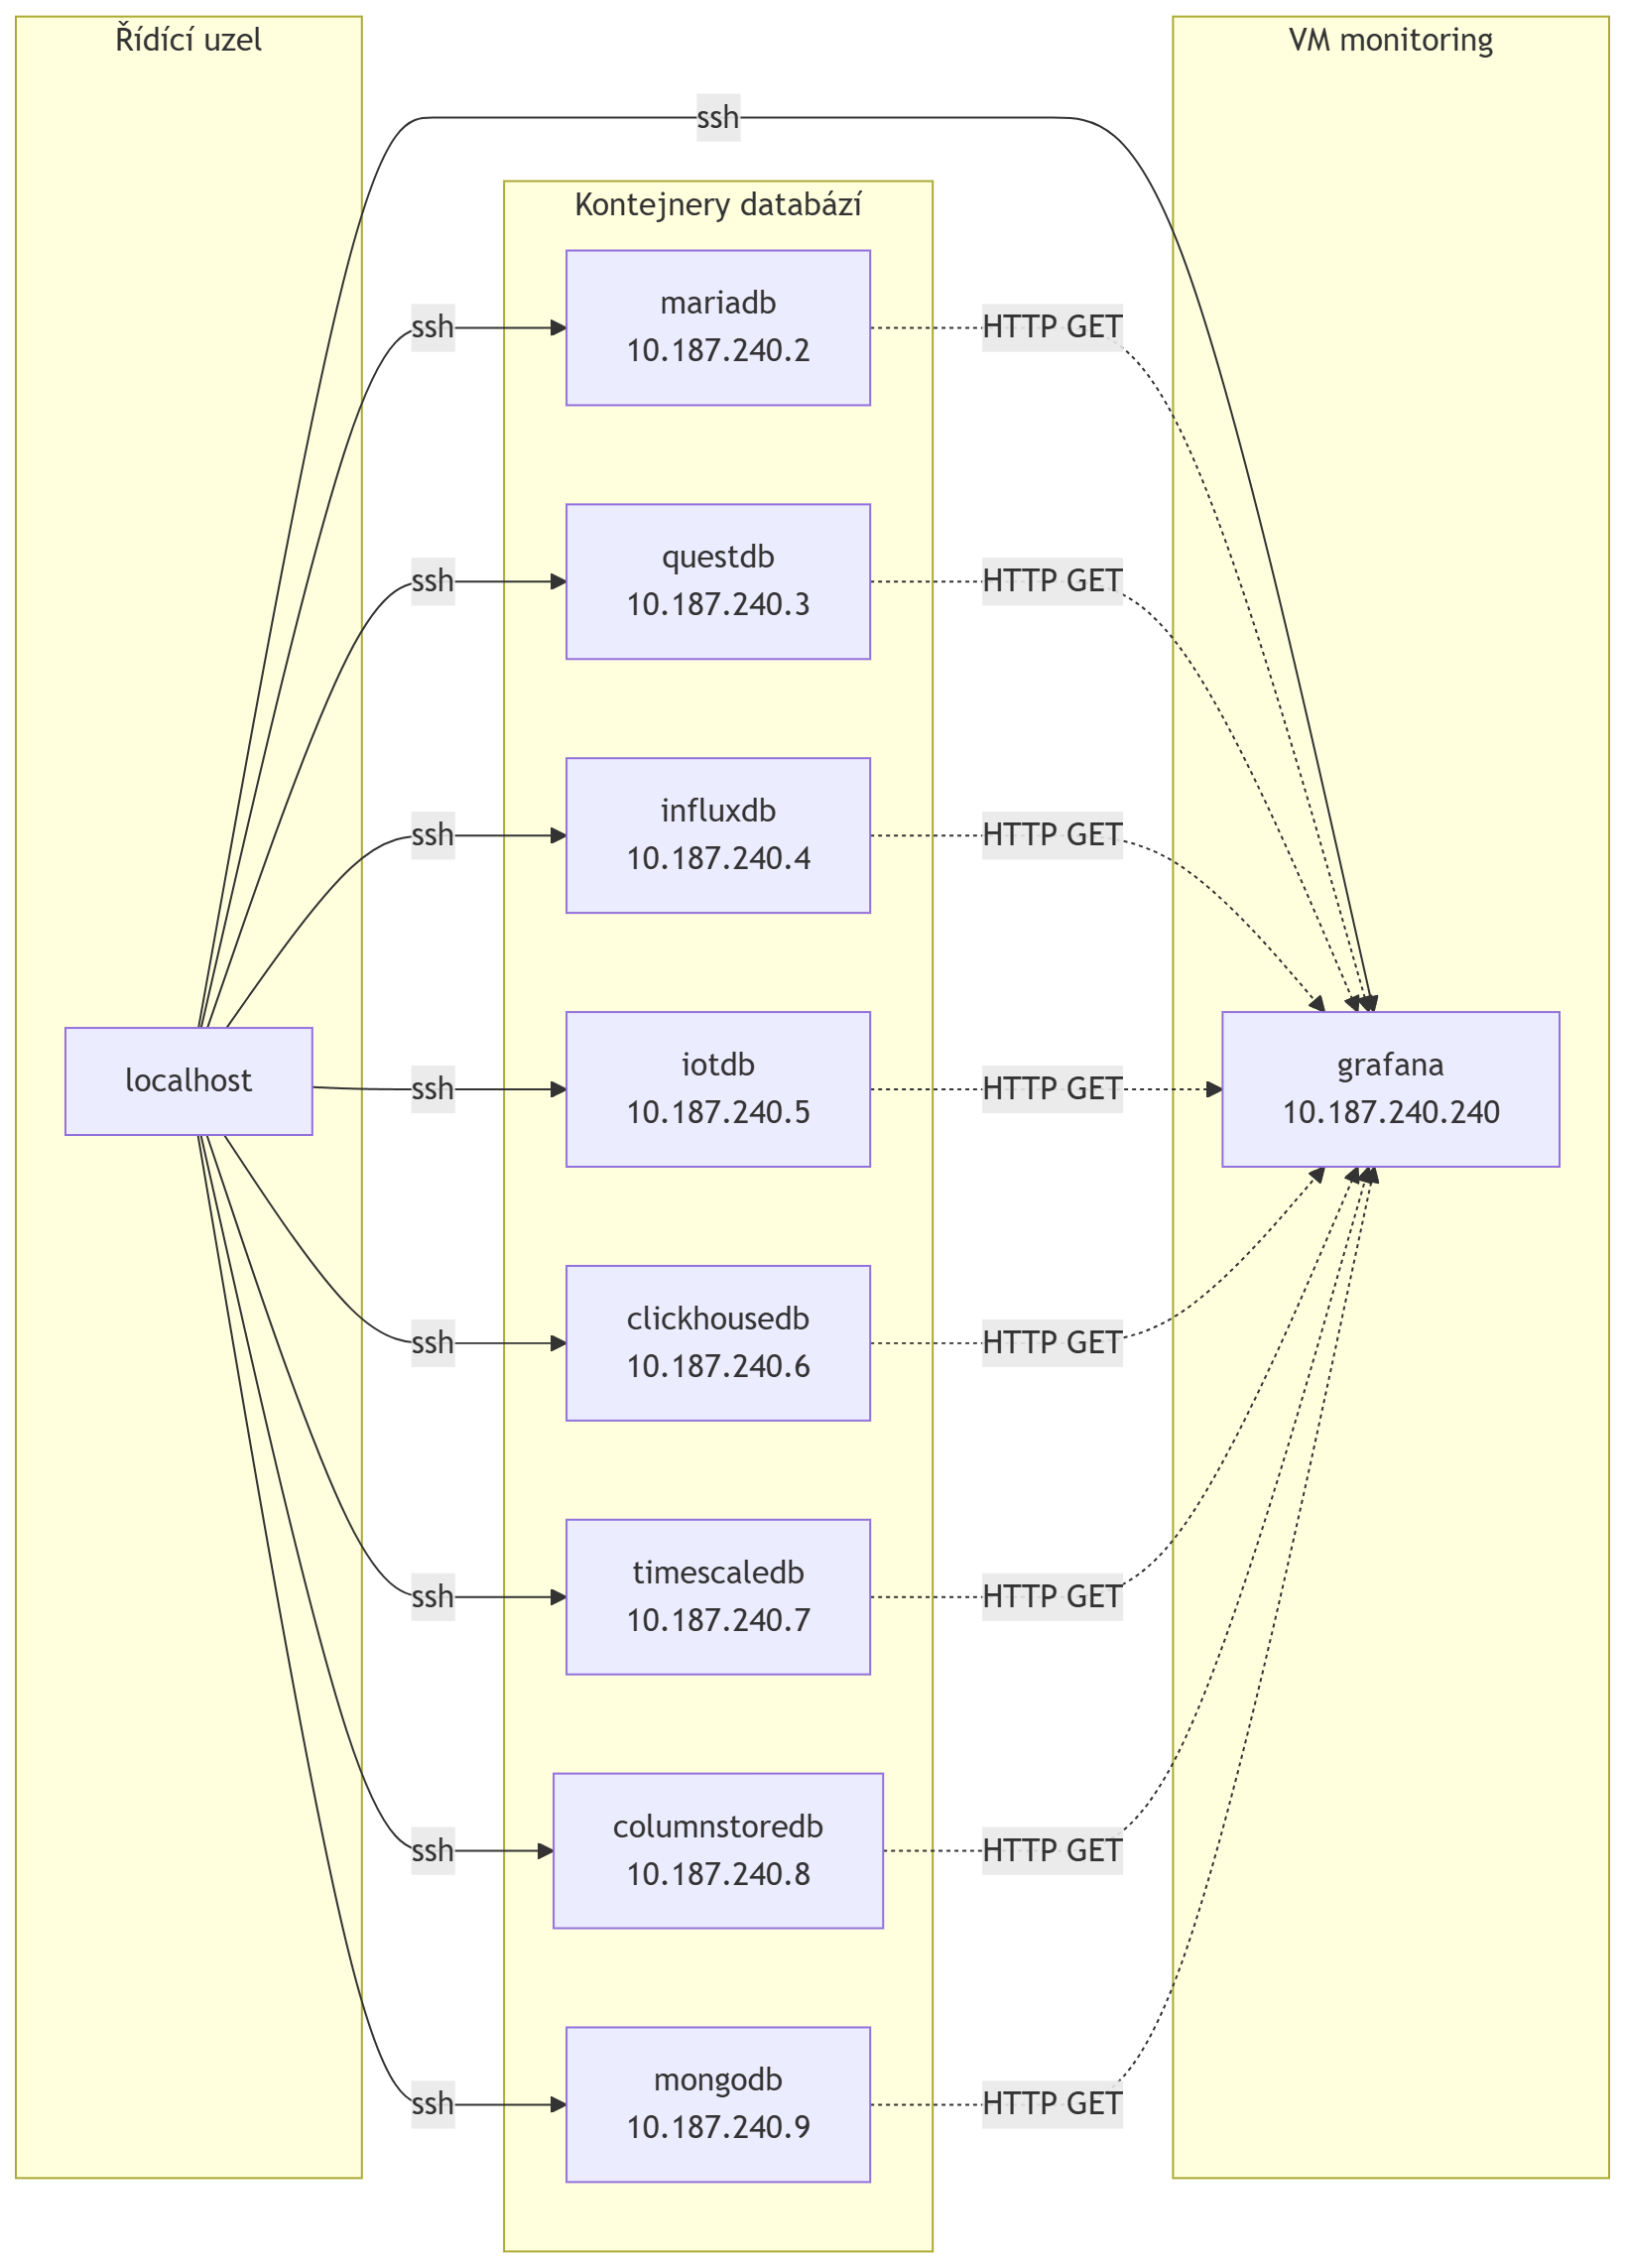
\includegraphics[width=0.6\textwidth]{images/architektura.png}
    \caption{Ukázka komunikace mezi uzly (zdroj: vlastní zpracování)}
    \label{fig:architektura}
\end{figure}
\clearpage
\subsection{Konfigurace databází}
\label{sec:rolecommon}

Každý databázový systém má vlastní roli ve stejné struktuře: \texttt{defaults/main.yml} definuje proměnné, \texttt{tasks/main.yml} pouze zřetězí instalaci a~konfiguraci, a~samotná logika je rozdělena do jednotlivých \texttt{tasks/*.yml}. 
Jako reprezentativní příklad je níže rozebrána role \texttt{clickhousedb}.

\subsubsection{Proměnné role}
Výchozí proměnné v~\texttt{roles/clickhousedb/defaults/main.yml} definují jak parametry pro vytvoření LXD instance, tak parametry samotné databáze:

\begin{lstlisting}[language=YAML, caption={Výchozí proměnné role clickhousedb}, label={lst:chdefaults}, captionpos=b]
keyring: "/usr/share/keyrings/clickhouse-keyring.gpg"
import_dir: "/var/lib/clickhouse/user_files"

vm_name: "clickhouse"
vm_packages:
  - apt-transport-https
  - ca-certificates
vm_disk_size: 6GB

data_file: ######

db_host: localhost
db_port: 9000
db_table: car_telemetry

db_key_url: "https://packages.clickhouse.com/rpm/lts/repodata/repomd.xml.key"
db_engine: "MergeTree"
\end{lstlisting}

\texttt{vm\_disk\_size} a~\texttt{vm\_packages} jsou čteny rolí \texttt{common-create} při~vytváření LXD instance, tedy ještě před tím, než se role \texttt{clickhousedb} vůbec spustí.
\clearpage
\subsubsection{Instalace databáze}
Soubor \texttt{tasks/install.yml} provede instalaci a~základní zprovoznění serveru:

\begin{lstlisting}[language=YAML, caption={roles/clickhousedb/tasks/install.yml (zkráceno)}, label={lst:chinstall}, captionpos=b]
- name: Download GPG key
  ansible.builtin.apt_key:
    url: "{{ db_key_url }}"
    keyring: "{{ keyring }}"
    state: present

- name: Add ClickHouse repository
  ansible.builtin.apt_repository:
    repo: >
      deb [signed-by={{ keyring }} arch=amd64]
      https://packages.clickhouse.com/deb lts main
    filename: clickhouse
  register: repo_result
  until: repo_result is succeeded

- name: Install ClickHouse packages
  ansible.builtin.apt:
    name: [clickhouse-server, clickhouse-client]
    state: present
    update_cache: true
  environment:
    DEBIAN_FRONTEND: noninteractive
  until: result is succeeded

- name: Ensure ClickHouse listens on all interfaces
  ansible.builtin.copy:
    dest: /etc/clickhouse-server/config.d/listen.xml
    content: |
      <yandex>
          <listen_host>0.0.0.0</listen_host>
      </yandex>
  notify: Restart ClickHouse

- name: Enable and start ClickHouse service
  ansible.builtin.service:
    name: clickhouse-server
    enabled: true
    state: started
\end{lstlisting}

Z~výpisu uvedeného konfiguračního souboru \ref{lst:chinstall} jsou patrné následující bloky:

\begin{itemize}
  \item \textbf{Download GPG key} - stažení GPG\footnote{\textit{GPG Key} - kryptografický klíč používaný k~ověření identity a~podepisování či~šifrování dat} klíče pro ověření balíčků z~repozitáře ClickHouse.
  \item \textbf{Add ClickHouse repository} - přidání repozitáře do systému, aby bylo možné instalovat balíčky \texttt{clickhouse-server} a~\texttt{clickhouse-client}.
  \item \textbf{Ensure ClickHouse listens on all interfaces} - přepsání výchozí konfigurace tak, aby služba ClickHouse poslouchala na všech síťových rozhraních.
  \item \textbf{Enable and start ClickHouse service} - povolení a~spuštění služby ClickHouse.
\end{itemize}

Výchozí konfigurace ClickHouse poslouchá pouze na loopback rozhraní\footnote{\textit{Loopback rozhraní} - síťové rozhraní, které umožňuje komunikaci pouze v~rámci stejného zařízení}, proto je nutné změnit konfigurační soubor \texttt{config.d/listen.xml} a~přepsat chování na adresu \texttt{0.0.0.0}, bez této úpravy by nebylo možné se serverem komunikovat mimo samotný kontejner. 
Změna konfiguračního souboru je navázána na handler, který po jejím zápisu ClickHouse restartuje:

\begin{lstlisting}[language=YAML, caption={roles/clickhousedb/handlers/main.yml}, label={lst:chhandlers}, captionpos=b]
- name: Restart ClickHouse
  ansible.builtin.service:
    name: clickhouse-server
    state: restarted
\end{lstlisting}

\subsubsection{Vytvoření datové struktury}
Po instalaci vytvoří \texttt{tasks/setup\_database.yml} cílovou tabulku pomocí příkazového klienta \texttt{clickhouse-client}. 
Tabulka odpovídá struktuře testovaného datasetu (viz sekce \ref{sec:popisdat}) a~je definována s~ohledem na typický přístup k~datům, dotazy filtrující podle vozidla a~času:

\begin{lstlisting}[language=YAML, caption={Výřez z~roles/clickhousedb/tasks/setup\_database.yml}, label={lst:chschema}, captionpos=b]
CREATE TABLE IF NOT EXISTS {{ db_table }}
(
    orig_time      DateTime64(9, 'Europe/Prague'),
    GpsTime        DateTime64(9, 'Europe/Prague'),
    VehicleID      String,
    Longitude      Decimal(14,10),
    Latitude       Decimal(14,10),
    SpeedGps       Decimal32(3),
    ...
)
ENGINE = {{ db_engine }}
ORDER BY (VehicleID, GpsTime)
PARTITION BY toDate(GpsTime)
PRIMARY KEY (VehicleID, GpsTime)
\end{lstlisting}

Klíč řazení (\texttt{ORDER BY}) a~primární klíč jsou zvoleny jako dvojice (\texttt{VehicleID}, \texttt{GpsTime}), díky čemuž jsou data uvnitř jednotlivých částí fyzicky uspořádána podle vozidla a~času.
Členění podle dne (\texttt{toDate(GpsTime)}) zároveň umožňuje ClickHouse při~dotazech s~časovým omezením přeskočit celé sekce, které se v~daném rozsahu nevyskytují.

Role \texttt{clickhousedb} tímto nijak nezasahuje do vytváření samotného virtuálního stroje, to má na starosti obecná role \texttt{common-create}, která nejprve deleguje výběr hardwarového profilu na roli \texttt{profile-loader}, poté vytvoří LXD instanci a~nakonec vyčká, než bude cíl dostupný přes SSH. 
Role databáze se tak spouští až nad již běžícím a~připraveným systémem, což umožňuje stejný postup jednotně opakovat pro všech osm testovaných systémů, liší se ovšem jednotlivé kroky při~instalaci a~vytvoření databází.

\section{Pilotní nasazení systémů}

Cílem pilotního nasazení nebylo měřit výkon, ale ověřit, že je celý navržený postup, vytvoření kontejneru, instalace databáze, import datasetu a~spuštění testovacích dotazů, funkční v~celé své šíři, dříve než bude spuštěn na cílové infrastruktuře poskytovatele dat.

Vzhledem k~omezené kapacitě notebooku nebylo možné provozovat všech osm databázových kontejnerů současně. 
Pilotní testování proto probíhalo postupně, vždy s~jedním běžícím databázovým strojem, přičemž ostatní byly po dobu testu vypnuty (role \texttt{common-stop}), stejný princip následně převzal i~produkční skript \texttt{run\_test.sh} (sekce \ref{sec:implementacetestu}).

Pilotní nasazení proběhlo ve dvou fázích:
\begin{itemize}
    \item \textbf{Manuální ověření} \\
    V~první fázi byl celý postup pro ClickHouse odzkoušen manuálně, přímými příkazy nad LXD (\texttt{lxc launch}, \texttt{lxc exec}) a~databázovým klientem. 
    Instalace balíčků, přidání repozitáře, vytvoření testovací tabulky, import datového souboru a~ověřovací agregační dotaz (\texttt{SELECT sum(SumSalt)...}) sloužily k~potvrzení, že zvolený formát dat, schéma tabulky i~způsob importu odpovídají očekávání, než byly zakomponovány do Ansible role.
    
    \item \textbf{Automatizované ověření} \\
    Po manuálním ověření byl stejný postup přepsán do role \texttt{clickhousedb} a~spuštěn přes \texttt{ansible-playbook}. 
    Kontejner byl mezi jednotlivými pokusy vždy odstraněn (\texttt{lxc delete <database>}) a~znovu vytvořen automatizovaně, čímž bylo potvrzeno, že celý proces je opakovatelný a~nezávislý na předchozím stavu systému.
\end{itemize}

Tento dvoufázový přístup byl následně zopakován i~pro zbývající databázové systémy a~stal se šablonou pro strukturu všech rolí v~adresáři~\texttt{roles/}, nejprve manuální ověření instalačního postupu dané databáze, poté jeho přenesení do role. 
Výstupem pilotní fáze tedy nebyla naměřená data, ale funkční a~opakovatelná automatizace, na jejímž základě mohlo být spuštěno systematické testování popsané v~následující sekci.
\clearpage
\section{Implementace testů}\label{sec:test_implementation}
Pro testování databázových systémů byly vytvořeny následující sady testů:
\begin{itemize}
    \item \textbf{Insert test} \\
    Test zaměřený na měření rychlosti zápisu dat do databáze.
    \item \textbf{Single point test} \\
    Test zaměřený na měření rychlosti vrácení jednoho specifického záznamu z~databáze.
    \item \textbf{Condition test} \\
    Test zaměřený na měření rychlosti vrácení všech záznamů splňujících určitou podmínku.
    Jako podmínku jsem si zvolil vrácení všech záznamů, které mají polohu v~určitém geografickém rozsahu za určité období.
    \item \textbf{Aggregate test} \\
    Test zaměřený na měření rychlosti provedení agregačního dotazu nad databází.
    V~agregačním testu jsem zvolil dotaz, který vrací průměrnou rychlost, maximální rychlost a~počet záznamů pro každé vozidlo za určité období.
\end{itemize}
Všechny tyto testy se spouští pomocí skriptu \texttt{run\_test.sh}, který přijímá následující parametry: 
\begin{itemize}
    \item -database|-d -- vybraný databázový systém
    \item -test\_type|-test|-t -- vybraný test
    \item -inventory|-i -- ansible inventář
    \item -profile|-p -- hardwarový profil
    \item -repeat|-r -- počet opakování
\end{itemize}

\vspace{1.5em}
\begin{lstlisting}[caption={Příklad spuštění live insert testu}, label={lst:liveinsert}, captionpos=b]
    ./run_test.sh -d clickhousedb -t insert -p medium -i remote -r 33 
\end{lstlisting}
\begin{itemize}
     \item \textbf{Live insert test} \\
    Test zaměřený na měření rychlosti zápisu dat v~reálném čase, kdy se do databáze kontinuálně vkládají nové záznamy.
    
    Spolu se stejnýmy parametry jako předešlé testy má i své speciální parametry:
    \begin{itemize}
        \item -workers|-w -- počet paralelních zdrojů, které vkládají data do databáze
        \item -duration|-t -- celková doba v~sekundách, po kterou bude test probíhat
        \item -batch\_size|-b -- počet záznamů v~jedné dávce, která bude vložena do databáze 
        najednou
        \item -step|-s -- časová mezera ve vložených datech
    \end{itemize}
    \clearpage
    Test se zavolá následujícím způsobem:
    \begin{lstlisting}[caption={Příklad spuštění live insert testu}, label={lst:liveinsert}, captionpos=b]
    ./run_live_insert.sh -d iotdb -i remote -p small -w 10 -dur 60 -b 50000 -s 1000 -r 5
    \end{lstlisting}
    Příkaz nastavý test pro databázový systém Apache IoTDB přes parametr \texttt{-d}, počet zdrojů na 4 přes parametr \texttt{-w}, dobu trvání testu na 60 sekund přes parametr \texttt{-t} a~velikost dávky na 1000 záznamů přes parametr \texttt{-b}. Dále nastaví inventář na \texttt{remote} a hardwarový profil na \texttt{small}. Celý test se bude opakovat 5$\times$.
\end{itemize}

Testování probíhalo na dvou prostředích: lokálně na vývojovém notebooku a~vzdáleně na serveru v~datovém centru poskytovatele DCÚK, kam je přístup realizován přes šifrované VPN\footnote{\textit{VPN (Virtual Private Network)} - technologie, která umožňuje bezpečné připojení ke vzdálené síti} připojení. Pro představu o~výpočetním kontextu uvádím srovnání klíčových hardwarových parametrů obou strojů v~tabulce \ref{tab:hardwarespecs}.

\begin{table}[H]
\centering
\caption{Porovnání hardwarových specifikací testovacích strojů}
\label{tab:hardwarespecs}
\begin{tabular}{@{}lcc@{}}
\toprule
\textbf{Parametr} & \textbf{Notebook} & \textbf{Server} \\
\midrule
Procesor & AMD Ryzen 5 5600H & Intel Xeon E5-2630 v3 \\
Jádra / vlákna & 6 / 12 & 8 / 16 \\
Max.\ frekvence & 4,2 GHz & 2,40 GHz \\
Mezipaměť L3 & 16 MB & 20 MB \\
Operační paměť & 16 GB DDR4-3200 & 125,69 GB DDR4-ECC 3200 \\
Úložiště & 512 GB NVMe M.2 SSD & 1,92 TB Micron SATA SSD \\
OS & Ubuntu 22.04 LTS (server) & Proxmox VE 9.0.11 \\
Jádro & Linux 6.8.0-134-generic & Linux 6.14.11-4-pve \\
\bottomrule
\end{tabular}
\end{table}

\subsection{Architektura spouštění testů}
\label{sec:implementacetestu}

Spuštění libovolného testu je řízeno jediným playbookem \texttt{tests/test.yml}, který se skládá ze dvou částí. 
První část zajistí, že cílová databáze běží (role \texttt{common-start}, která se v~případě neexistujícího virtuálního stroje sama pokusí o~jeho vytvoření rolí \texttt{common-create}). 
Druhá část se připojí přímo na databázový host, vyčká na dostupnost databáze a~poté vloží konkrétní testovací úlohu podle proměnných \texttt{database} a~\texttt{test\_type}:

\begin{lstlisting}[language=YAML, caption={Výřez z~tests/test.yml}, label={lst:testyml}, captionpos=b]
tasks:
  - name: Start {{ database }} - {{ test_type }}
    ansible.builtin.include_tasks:
      file: "{{ database }}/{{ test\_type }}.yml"

post_tasks:
  - name: Common Post Processing
    ansible.builtin.include_role:
      name: common-post-processing
\end{lstlisting}

Díky tomuto vzoru obsahuje adresář \texttt{tests/} pro každou databázi pět souborů se stejným názvem jako typ testu:
\begin{itemize}
    \item \texttt{insert.yml}
    \item \texttt{single\_point.yml}
    \item \texttt{condition.yml}
    \item \texttt{aggregate.yml}
    \item \texttt{live\_insert.yml}
\end{itemize}

Tyto testy obsahují databázově specifický dotaz, ale vracejí shodnou sadu faktů (\texttt{start\_datetime}, \texttt{host}, \texttt{rows\_returned}, atd.), se kterou dále pracuje role \texttt{common-post-processing}.

\subsubsection{Hardwarové profily}

Pro možnost testování vlivu výpočetních prostředků na výkon databázových systémů byly definovány tři hardwarové profily. Každý kontejner je při vytvoření nakonfigurován podle zvoleného profilu, který určuje limit operační paměti a počet dostupných procesorových jader:

\begin{lstlisting}[language=YAML, caption={Definice hardwarových profilů}, label={lst:profiles}, captionpos=b]
profiles:
  small:
    ram_limit: "2GiB"
    cpu_limit: "1"

  medium:
    ram_limit: "4GiB"
    cpu_limit: "2"

  large:
    ram_limit: "8GiB"
    cpu_limit: "4"
\end{lstlisting}

Při spuštění testu je profil vybrán proměnnou \texttt{profile}, která je předána roli \texttt{common-create}. Ta na jejím základě přidělí kontejneru odpovídající prostředky.

\subsubsection{Měření doby trvání dotazu}
Pro testy \textit{single point}, \textit{condition} a~\textit{aggregate} nebyla doba trvání měřena na straně Ansible (tj. jako čas mezi odesláním a~přijetím SSH příkazu), ale přímo na straně databázového serveru. 
U~ClickHouse je každý dotaz spuštěn s~explicitním \texttt{--query\_id}, jehož hodnota je následně vyhledána v~systémové tabulce \texttt{system.query\_log}:

\begin{lstlisting}[caption={Výřez z~tests/clickhousedb/helper/get\_query\_timing.yml}, label={lst:getquerytiming}, captionpos=b]
SELECT
  query_duration_ms,
  read_rows,
  result_rows
FROM system.query_log
WHERE type = 'QueryFinish'
  AND query_id = '{{ clickhouse_query_id }}'
LIMIT 1
\end{lstlisting}

Tento přístup, opakovaný s~krátkým prodlením až do maximálního počtu pokusů (dotaz se v~\texttt{query\_log} objeví až po jeho dokončení a~krátkém interním zpoždění), odstraňuje z~naměřené hodnoty režii SSH spojení a~síťovou latenci mezi řídicím strojem a~testovaným kontejnerem, naměřený čas tak odpovídá čistě době zpracování dotazu databázovým enginem.

Test \textit{insert} je naopak měřen na straně shellu pomocí nástroje \texttt{/usr/bin/time}, protože importovaná data se do \texttt{system.query\_log} zapisují jako jediný (dlouho běžící) dotaz a~jeho reálná doba trvání zahrnuje i~čtení a~dekompresi vstupního souboru:

\begin{lstlisting}[caption={Výřez z~tests/clickhousedb/insert.yml}, label={lst:chinsert}, captionpos=b]
/usr/bin/time -f "DURATION\_SECONDS=%e" \
sudo clickhouse-client \
  -q "INSERT INTO {{ db_table }} FORMAT CSVWithNames" \
  < {{ import_dir }}/{{ data_gz }}
\end{lstlisting}

\subsubsection{Live insert test}
Test v~reálném čase je jediný, který není implementován jako jednorázový SQL příkaz, ale jako samostatný Python skript nasazený na cílový virtuální stroj. 
Sdílené soubory \texttt{generate\_live\_data.py}, \texttt{runner.py} a~\texttt{base\_driver.py} jsou společné pro všechny databáze a~definují abstraktní rozhraní ovladače (počet workerů, batch size a~interval měření). 
Konkrétní implementace zápisu pro danou databázi (např. přes knihovnu \texttt{clickhouse-driver}) je uložena v~\texttt{tests/\{database\}/driver.py} a~je na virtuální stroj zkopírována až podle proměnné \texttt{database}:

\begin{lstlisting}[caption={Výřez z~tests/clickhousedb/live\_insert.yml}, label={lst:liveinserttask}, captionpos=b]
- name: Deploy {{ database }} driver to VM
  ansible.builtin.copy:
    src: "{{ project_root }}/tests/{{ database }}/driver.py"
    dest: "{{ bench_dir.path }}/driver.py"

- name: Run live insert benchmark
  ansible.builtin.command: >
    python3 {{ bench_dir.path }}/runner.py
    --driver-path {{ bench_dir.path }}/driver.py
    --duration {{ duration }} --workers {{ workers }}
    --batch-size {{ batch_size }} --ts-step-ms {{ ts_step_ms }}
    --output {{ bench_dir.path }}/live_result.json
\end{lstlisting}

Skript \texttt{runner.py} rozdělí zadaný počet simulovaných vozidel rovnoměrně mezi \texttt{workers} paralelních procesů, po dobu \texttt{duration} sekund vkládá dávky o~velikosti \texttt{batch\_size} záznamů a~výsledek (celkový počet vložených řádků, statistiky za jednotlivé workery) uloží jako JSON. 
Ansible tento soubor po skončení testu stáhne zpět a~jeho hodnoty namapuje na stejnou sadu faktů, kterou používají ostatní testy, díky čemuž prochází live insert test stejnou post-processing logikou jako zbytek testovací sady.

\subsubsection{Sběr a~agregace výsledků}
Bez ohledu na typ testu je posledním krokem každého běhu role \texttt{common-post-processing}, která:
\begin{itemize}
    \item přečte konfiguraci virtuálního stroje uloženou při~jeho vytváření v~\texttt{/etc/vm\_config.json} (přidělený RAM, CPU a~použitý profil),
    \item sestaví jeden JSON záznam obsahující typ testu, cílovou databázi, čas začátku a~konce, dobu trvání, počet přečtených/vrácených řádků a~parametry profilu,
    \item tento záznam připojí jako nový řádek do souboru \texttt{results/\{test\_type\}.ndjson} na řídicím stroji,
    \item a~zapíše odpovídající anotaci do Grafany (\texttt{/api/annotations}), čímž se testovací okno zpětně promítne do grafů systémových metrik sbíraných Prometheem.
\end{itemize}

Tímto způsobem vznikne za všechny databáze a~všechny opakované běhy jednotná sada pěti NDJSON(Newline Delimited JSON) souborů (\texttt{insert}, \texttt{single\_point}, \texttt{condition}, \texttt{aggregate}, \texttt{live\_insert}), která slouží jako vstupní data pro následnou analýzu výsledků.

Ze všech testů se sbírají metriky dvojím způsobem:
\begin{itemize}
    \item \textbf{NDJSON výsledky} \\
    Po dokončení každého testu se výsledky ukládají do souboru ve formátu NDJSON, který obsahuje informace o~době trvání dotazu, počtu záznamů vrácených dotazem...
    \item \textbf{Prometheus metriky} \\
    Během testů se v~každém kontejneru sbírají metriky pomocí Node Exporteru, které jsou následně shromažďovány službou Prometheus. 
    Tyto metriky zahrnují využití CPU, využití paměti, I/O~operace disku a~síťovou aktivitu.
\end{itemize}